

\chapter{Analysis}

In this chapter, look at the current state-of-the-art. 
We examine standard shell features because they represent both what people are used to and the starting point for our solution.

Because we want to know who we design for we introduce target users for our future design. We formulate shell history workflows based on shell usage data we collected from several people. %Each workflow is described in detail. 
These workflows show us when standard shell history features work well and when there are issues. We explain the limitations and disadvantages of standard shell history features.

After that, we review existing history tools to see what problems they solve. We identify tools that solve the issues of standard shell history features. We also find contextual history tools that do not bring much value to the user.

Then, we explore what contextual information is available in shell. We break it down into multiple distinct categories. For each category, we describe how it relates to shell usage and how could it be useful in history tools.


\section{Standard shell history features}

In this section, we describe common shell history features of Bash\cite{bashman} and Zsh\cite{zshdocs}. Most of these features are enabled by default so the user does not have to configure them before using them.
%These features are most likely available to the majority our target users. %Standard shell history features shape how people use shell history. 
For each of the features we point out its advantages and disadvantages.
The list of history features we cover is following:

\begin{itemize}
    \item Saving history entries
    \item History substitution
    \item Stepping through recent history
    \item Prefix search
    \item Reverse search
    \item Manual history filtering
\end{itemize}


\subsection{Saving history entries}

%First, we take a look at how command line entries are saved into history.
Whenever you submit a command line entry in shell it is added to history. Saved history entries are then available for future reuse. %We describe specific ways to access the history a bit later.

It is possible to configure shell to not save duplicate entries to history.  
In Zsh, we can also keep duplicates in history but prevent them from showing up when searching.  
There are options to prevent specific command line entries from being saved to history based on a user specified pattern. %This is done using \verb|HISTIGNORE| option in Bash.

We can configure shell history to save time of the execution alongside the history entry. In Zsh, it is also possible to record and save duration of the execution.

\paragraph{Missing history entries}

When we execute a command line entry we generally expect to be able to find it in history. This is not always the case. There are multiple reasons why executed command line entries can be missing in the shell history.

In Bash, simultaneous terminal sessions can overwrite the history of one another when it is being written to disk.\cite{bashman}\cite{bash-session-issues-1} This can be prevented by properly configuring the shell.

Shell history is not unlimited. We might not be able to find history entries simply because they are too old and our history size is too small. Size of shell history can be increased with configuration options. % \verb|HISTSIZE| and \verb|SAVEHIST| or \verb|HISTFILESIZE|.

\subsection{History substitution}

History substitution is a powerful feature that allows users to reuse previous history entries or their parts. 
For example, we can use \verb|!!| to repeat previous history entry and \verb|!$| to repeat its last argument. Executing a history entry based on its absolute or relative index can be done using \verb|!5| or \verb|!-2| respectively.

The flexible notation of history substitution makes it possible to match recent history and perform substitutions on them. For instance, \verb|!cc| executes the last history entry that starts with \verb|cc|. An example of substitution is \verb|!!:s/foo/bar/|; It retrieves the previous history entry and replaces instances of \verb|foo| with \verb|bar|.

History substitution is powerful and flexible but it is non-interactive. Users do not know what the substitution evaluates to until they execute it. For example, submitting \verb|!rm| could lead to a irreversible losses.

It is possible to configure shell to show us the result of the substitution before executing it. Doing so however, adds extra step to each history substitution we perform. The additional required interaction can be very annoying in simple cases such as \verb|sudo !!|. A less invasive way to evaluate the substitutions before execution is \verb|magic-space|; It causes shell to expand substitutions after we press \verb|SPACE|.

\subsection{Stepping through recent history}

Repeatedly pressing \verb|ARROW_UP| gives us access to immediately previous history entries. Conversely, we can press \verb|ARROW_DOWN| to get back to the original command line. 

This is very quick and convenient way to access recent history entries. Instead of trying to remember the previous history entries we can interactively step through them.

Quite obviously this is not a great way to access older than recent history entries. Pressing \verb|ARROW_UP| many times and reading the results as they appear can take considerable amounts of time.

\subsection{Prefix search}

Prefix search works similarly as stepping through history using \verb|ARROW_UP|. It returns previous history entries that match the prefix we have already typed. 
This enables us to reuse recent and even older history entries based on their prefix. Prefix search is convenient in practice; For example, we can search for previous \verb|git| commands which all most likely start with \verb|git| prefix.

When there is no prefix, prefix search works just like simple stepping through recent history. Because of that it can be bound to \verb|ARROW_UP|, \verb|ARROW_DOWN| and used as a reasonable replacement for the default behavior. We can find prefix search configured this way in a popular Zsh configuration framework -- Oh-my-zsh\cite{toolsohmyzsh}.

In both Bash and Zsh, prefix search is not configured by default. Before we people can start using it, they need to find out that it exists and configure it. This is one of many examples where we can see the importance of good defaults; Many people only know the default state of the shell because they never change the default configuration.

\subsection{Reverse search}

With prefix search, we could only search the history by prefix.
Reverse search allows us to interactively search for previous history entries based on any part of the command line entry. It can be activated using \verb|CTRL-R|.

In contrast to prefix search, reverse search is available by default and people seem to use it a lot. Reverse search is the most powerful interactive history search feature included in Bash and Zsh.

Reverse search might seem like the perfect way to search history. However, it does have its limitations. First, we cannot search using more than one word. In other words, the search query needs to be consecutive. Second, only one result is displayed at a time. We need to repeatedly press \verb|CTRL-R| to see more results.

Pointing out these limitations might seem like nitpicking. However, we will see later that they do limit the searching capabilities of reverse search significantly.


\subsection{Manual history filtering}

Shells offer builtin commands to print and control history. Builtin command \verb|history| and standard shell utilities can be used for powerful history searching.
For example, running \verb#history | grep 'pattern1' | grep 'pattern2'# prints the searches the history using two words and displays all matching results.

Manually filtering history overcomes the limitations of reverse search. However, extra typing is necessary to complete the searches compared to interactive methods. Plus, unlike with reverse search, we cannot see the results update as we type the search query.


\section{Target users}

When designing any product, we need to make sure we know who the product is for. Shell history tools are no exception. To capture the target user-base we are modelling two typical users as personas.% As the first persona we chose an experienced user because shell history tools are likely more for users that use shell extensively. As the second persona we chose a novice shell user; Designing tools for novice shell users can result in a product that is better for everyone. For example, it is especially important for novice users that the product is easy to install, comes with a good default configuration, and is easy to use for the first time; These characteristics are beneficial to everyone not just novice users. 

\subsection{Typical experienced shell user}

Experienced professional programmer \textit{Peter} develops, deploys, and operates back-end applications. Main languages he uses at work are C and C++. He has years of experience with developing on and for the Linux operating system. He is proficient in Bash and he has written a few small shell scripts to increase his productivity.

His editor of choice is Vim; He has a sizable Vim configuration with multiple Vim plugins he collected over the years.

The shell he uses is Zsh with Oh-my-zsh \cite{toolsohmyzsh} shell configuration framework. On top of that he maintains a set of his own custom options and aliases. He puts the resulting configurations on his machines. He does not change his configuration often but he likes to be able to configure his shell and other tools he uses.

He often uses \verb|ssh| to log into remote machines; The remote machines are shared and have the default shell configuration. He keeps his shell and editor configuration somewhat similar to the default one because he does not want to constantly switch between very different environments. 

His daily shell workflows include complex commands with many long arguments and switching between many different projects. When coming back to a project he sometimes cannot remember what command line entries he was using. He is familiar with Make but he often forgets to create Makefiles for typical tasks in projects.

He makes use of interactive history features like reverse search and prefix search. However, he quite often uses \verb#history | grep 'pattern1' | grep# \verb#'pattern2'# to manually filter shell history because it is both more powerful and sometimes feels easier to use than reverse search. Manual filtering allows him to search by more than one pattern and to see many of the matching results. 

%\todotext{TODO: ADD challenges and benefits ? maybe}

\subsection{Typical novice shell user}

Junior data analyst \textit{Mark} has recently started his first job. He uses shell because he needs it at work. The primary language he uses is Python. 

The editor he uses is Visual Studio Code because it was recommended to him by a coworker. He likes that it suggests extensions to install based on files he is working with.

He is using Bash with the default configuration provided by Ubuntu distribution; Apart from that he does not have any custom shell configuration. 

Since he does not have much experience with shells, he neither does understand the shell configuration files nor he feels confident editing them. If he discovered or someone recommended a new shell tool to him he would prefer an installation without the need to edit the shell configuration files. Additionally, he expects any programs and tools he installs to work out-of-the-box and not to require much configuration. 

There are shell history features he is not aware of like history expansion and prefix search. He uses arrow keys to get recently submitted command line entries and he presses \verb|CTRL-R| when looking for history entries further in the past. 

%\todotext{TODO: ADD challenges and benefits ? maybe}


\section{Common shell history workflows}

Now that we know who our target users are we can formulate common workflows for them. Workflows are formulated based on interviewing user, collected shell usage data\footnote{We have collected shell history and usage data from a few people with different experience levels. We used this data to confirm the workflows where possible.}, and our experience with shells. 

Some of the workflows can be easily fulfilled using standard history features. Others are either difficult or impossible to complete. We describe and explain the issues people can encounter when using standard history features. The list of workflows we cover is following:

%We do not specify the workflows for each of the target users separately; Instead, we comment on the difference between the users when necessary. \todo{we only ever make comments about the experience level of the users}

%Workflows we formulate are based on previous research \cite{greenberg1993computer}, the online discourse we discussed earlier, discussions with potential users, and our own experience with shell history. Additionally, we collected and examined shell usage and history of a few users; This helped us to confirm and formulate the workflows.

%\todotext{Workflows are simplified by using common commands to make them easy to understand. Some of them were shortened to fit onto the page. Real examples would contain commands specific to the individual users work and the command line submissions would be longer in some cases.}

%\redtext{There is one more thing you should keep in mind when reading the examples; You, unlike the user, will have the full sequence of history entries in front of you. The user in the examples will often have only limited memory of the command line entries he submitted earlier. }



%\redtext{We grouped the workflows to several distinct categories; In each category we explain the  ...}
%\redtext{In this section, we discuss how the users can complete these workflows using standard shell history features. We also point out the limits and shortcomings of the standard history mechanisms. }

\begin{itemize}
    \item Editing an immediately preceding history entry
    \item Blindly recalling very recent history entries
    \item Retrieving recent history entries
    \item Editing recalled history entries
    \item Repeating a sequence of history entries
    \item Searching with limited knowledge
    \item Searching with implicit context
\end{itemize}

%Additional configurations and tools will be discussed in later sections.

\subsection{Editing an immediately preceding history entry}

In this first workflow, the user submits a command line entry but is not satisfied with the result. To fix that, he retrieves the immediately preceding history entry, modifies it and executes it again. We will look at multiple example sequences of command line submissions for this workflow.

\begin{verbatim}
    wget https://pastebin.com/raw/EDELXNYp --silent
    wget https://pastebin.com/raw/EDELXNYp --quiet
\end{verbatim}
In this example, the user is trying to download a file from \verb|pastebin| using \verb|wget|. The first command ends with a non-zero exit status because \verb|--silent| is not an option of \verb|wget|. He presses \verb|ARROW_UP| to retrieve the previous command line entry, fixes the mistake and presses \verb|ENTER| to submit the command line entry again. 

Using \verb|ARROW_UP| is efficient in situations when we need to either edit the end of the command line entry or append to it. % Command line editing -> more efficiency
The next example shows a different case.

\begin{verbatim}
    apt-get install zsh
    sudo !!
\end{verbatim}

Here, the user wants to install the \verb|zsh| package. The command fails because superuser permissions are needed to install packages to the system. Instead of using interactive history features, the user uses history substitution \verb|!!| which repeats the previous history entry. 

By using \verb|!!| we can efficiently prepend or append to the previous command line entry. There are other csh-style history expansions but \verb|!!| is by far the most commonly used one. 

So far, we only saw situations where the submitted command line ended with a non-zero exit status and then the user fixed the error. This is not always the case because not all errors result in a non-zero exit code; Some errors are logical and not all programs respect the convention of properly signaling errors. Additionally, users sometimes gradually change and develop a command line entry to make sure that each step of the process works as intended. This is shown in the example below.

\begin{verbatim}
    sort data.txt
    sort data.txt | uniq -c
    sort data.txt | uniq -c > data_processed.txt
\end{verbatim}

In this next example, we see how the user processes \verb|data.txt| file. In each step, he uses \verb|ARROW_UP| to retrieve the previous history entry and continues editing it. When he is satisfied with the result, he redirects the processed data into a file. 

This example shows that there is not always an explicit error that could be detected by the shell to predict that the user will recall the previous history entry. It also shows that the editing process can be often continuous.

We just saw multiple different situations in which people continue working on the same command. We also saw different approaches to retrieving previous history entries. It is worth noting that in all of these situations the user relies on the order of the shell history. 

\subsection{Blindly recalling very recent history entries}

This second workflow is a retrieval and execution of a very recent history entry. Here, the user remembers the exact position of the history entry he wants to recall. An example of such workflow is running the following sequence of command line submissions.
\begin{verbatim}
    make build
    vim hello_world.c
    make build
\end{verbatim}
First, we use \verb|make| to build a project. Then we edit a file using \verb|vim|. After that, we press \verb|ARROW_UP| twice and press \verb|ENTER| to execute the recalled history entry -- \verb|make build|. 


Consider, if we used a graphical editor or if we ran the editor from a different terminal; In such case, we would only have to press \verb|ARROW_UP| once but the workflow would essentially stay the same.

When recalling very recent commands the users often remember the exact position of the history entry; This means that they do not read the history entry that appears on the command line but they blindly execute it instead. This is an efficient workflow that shows us the importance of the order of recent history entries.

\subsection{Retrieving recent history entries}\label{workflow-recent-history-arrow-up}
The third workflow is a retrieval of history entry that is still recent but the user no longer remembers the exact position in the history list. This means that the user needs to read the history entries as they appear to see if the desired entry was retrieved. This is an example sequence of command line entries for this workflow.

\begin{verbatim}
    systemctl start nginx.service
    systemctl status nginx.service
    tail /var/log/nginx/error.log
    nginx -t
    vim /etc/nginx/nginx.conf
    nginx -t
    systemctl start nginx.service
\end{verbatim}

In this example, the user is trying to start an Nginx \cite{reese2008nginx} web server. At first, the server does not start and the command returns an error. The user quickly realizes that there is an syntactic error in the configuration file after checking it using \verb|nginx -t|. Then, the configuration is fixed using \verb|vim| and the syntax is checked again using \verb|nginx -t|. 

At this point, the user presses \verb|ARROW_UP| five or six times\footnote{It could five or six depending on whether or not the user has history deduplication turned on.} to retrieve a recently executed command line entry \verb|systemctl start nginx.service|. Every time they press \verb|ARROW_UP| a single result appears and they need to read it. There is no way to tell if the desired result is one press of a button away, three, or seven. % When the user presses \verb|ARROW_UP| too many times they can show previous history entries by pressing \verb|ARROW_DOWN|.


% It seems that people experience the sunk cost fallacy\footnote{\redtext{TODO: describe?}} which combined with the lack of feedback from the system drives them to stick to the original plan -- pressing \verb|ARROW_UP|. 

You might think that people would not press \verb|ARROW_UP| five or six times and would rather use other history mechanisms.
However, the usage data we collected shows that even someone who claimed to not press \verb|ARROW_UP| excessively actually does so quite often. Pressing \verb|ARROW_UP| five times is more common than you would expect and pressing it over ten times is rare but it still happens. We also quite often saw people pressing \verb|ARROW_UP| too many times and then using \verb|ARROW_DOWN| to go back to previous history entries; We think that it is easy to overshoot when you only see one history entry at a time.

%\todo{we could include reasons why people do this but I don't think it's necessary/important (see drafts in comments)}

% 1-2 was the most common ... 5-6 quite common ... 8 - 10 rare  20 exceptions
% WHY: sunk cost fallacy + lack of feedback from the system
% WHY: people might not realize how far the entry is in the first place
% WHY: people do not want to "abandon the effort they have already put in" because anytime the result could be there

%It seems that in situations like this one people do remember the history entry well and perceive it as recent. This is why they chose to use  

\paragraph{Prefix search}

An efficient alternative way to fulfil the same workflow is to use history prefix search. To use prefix search the user needs to remember the first word or at least the first few characters of the command line entry; This is very likely since all the command line entries we are retrieving in this workflow are recent.

We will use the example with Nginx to compare using prefix search with simple stepping through recent history. When using prefix search, the user types in a prefix -- \verb|systemctl| -- and presses \verb|ARROW_UP| twice to get to the desired history entry. In contrast, when only using \verb|ARROW_UP| it took five or six presses to get to the history entry.

This might not seem like an improvement because we need to type the prefix before we start pressing \verb|ARROW_UP|. However, we have to realize that going through multiple history entries and reading them one by one requires a significant amount of time and effort compared to typing. 
    
This is a good example of how the number of keystrokes is not the only thing we should be taking into account; Generally speaking, shell history should save effort and time of its users. Retrieving previous history entries should be both mechanically and cognitively less demanding than typing them again.\cite{greenberg1993computer}

% REF(greenberg): Recurring inputs should be reentered more easily than the user's original entry, with the aim of reducing both physical tedium and the cognitive overhead of remembering past inputs. Reuse facilities should not be targeted only to experts, as they can help everyone.

% the prefix could be shorter e.g. "sys", "system"  ... typing vs. effort required to decide how long/short prefix is sufficient

%\todotext{Is this ending good? - continue (check comments)}

% ADD(polished?): There is a vocal group of people with strong preference for prefix search. The rest of the people either do not know that prefix search exists, do not have it configured, or prefer plain \verb|ARROW_UP| possibly out of habit.
% NOTE: maybe this^ belongs earlier? (but maybe not)


\subsection{Editing recalled history entries}

In the previous section, we saw a workflow where the user retrieved a recent history entry and executed it without any changes. Now, we are going to look at a similar workflow where the user retrieves a history entry, edits it and then executes it again. Workflows with editing are a little less common than the ones with direct execution according to the usage data we collected. An example of a workflow with editing follows.

\begin{verbatim}
    curl --data "value=test" http://localhost:8080/submit
    git add pkg/submit/submit.go
    git commit --message "fix submit endpoint"
    git tag v2.4.0-rc.1
    git push
    git push --tags
    curl --data "value=test" http://test.example.com:8080/submit
\end{verbatim}


Here, the user is using \verb|curl| to test a server endpoint running locally at \verb|localhost:3000/submit|. After being done with the testing he commits the changes, tags the version as a pre-release\footnote{Here "rc" in "v2.4.0-rc.1" version stands for release candidate which is sometimes used to mark pre-release versions.}, and pushes both commits and tags to the upstream. This triggers a CI pipeline that deploys the new version to testing environment. The user wants to test that the endpoint also works there.

At this point, the user presses \verb|ARROW_UP| six times to get to the desired history entry.\footnote{Alternatively, he could also use prefix search which would be more efficient.} 
After retrieving the desired history entry, the user needs to edit it to change the server URL from \verb|localhost| to \verb|test.example.com|. He holds down \verb|ARROW_LEFT| for a about a second, holds down \verb|DELETE| for about a second, types \verb|test.example.com|, and finally executes the changed command line entry. 

This seems a little tedious but it is still more efficient than typing the whole command line entry from scratch. Instead of navigating by and deleting single characters, we could use \verb|CTRL+ARROW_LEFT| to navigate by words and \verb|ALT+BACKSPACE| to delete whole words; This would be faster and more efficient. %However, it seems that many people do not use the command line editing functions.\todo{TODO: Ask more people, so far more people use it than I expected}

This workflow shows us how people edit history entries after they retrieve them. We see that standard history mechanisms make it possible to edit history entries after retrieval. %Reverse search, which we did not see in any workflow yet, is not an exception. 
This is a useful property that we should include in our designs as well. 

\subsection{Repeating a sequence of history entries}\label{workflow-repeating-a-sequence}

In this workflow, the user has executed a sequence of command line entries. He wants to retrieve and repeat all the command line entries in the sequence. 
Consider a following example.

\begin{verbatim}
    gcc generate_dot.c -o generate_dot.out
    ./generate_dot.out > graph.dot
    dot -Tpng -ograph.png graph.dot
    feh graph.png
    gcc generate_dot.c -o generate_dot.out
    ./generate_dot.out > graph.dot
    dot -Tpng -ograph.png graph.dot
    feh graph.png
\end{verbatim}

In this example, we are editing the \verb|generate_dot.c| file in another window. In current terminal, we compile a source file \verb|generate_dot.c|, generate a graph in the DOT\cite{graphvizthedotlanguage} language, run Graphviz\cite{ellson2001graphviz} command \verb|dot| to generate an image, and finally use image viewer \verb|feh|\cite{toolsfeh} to display the resulting image.

% ALT (too long): After observing the resulting image, we edit the source file \verb|generate_dot.c| in another window.
After observing the image, we edit the source file \verb|generate_dot.c| in another window.


Now, we want to repeat the whole process of generating the graph and view the resulting image. To retrieve the \verb|gcc| history entry, we press \verb|ARROW_UP| four times. Retrieving the next \verb|./generate_dot.out| entry also takes four presses of \verb|ARROW_UP|. Similarly, we need four key presses for each of \verb|dot| and \verb|feh| history entries. 

We need four key presses every time because with each executed command line entry we are pushing all the history entries further back in the history. We see that using \verb|ARROW_UP| to repeat a block of history entries is quite inefficient.  

There is other standard history mechanism we could use to repeat a block of history entries; 
Executing \verb|fc -4 -1| opens an editor with last four history entries and then, closing the editor executes the commands. This, however, is quite cumbersome in practice and not many people seem to use it. 

%Alternatively, we could use history expansion \verb|!-4| to recall and execute the fourth previous history entry; However, history expansion is not saved to 
%\todo{Consider mentioning history expansion (see comment)}
%\verb|!-4| works in a similar way

Repeating a sequence of history entries is not the most common workflow. However, it shows us the limits and inefficiencies of standard shell history.


\subsection{Searching with limited knowledge}\label{workflow-search-w-limited-knowledge}

In all the workflows we discussed so far, the user wanted to recall a fairly recent history entry. Now, we move on to workflows where the user searches for history entries that are older. In these workflows, the memory of the user is often a limiting factor; Both the knowledge of shell history and the desired command line entry is limited.

Below, we see an example for such workflow; The upper part contains relevant history entries from history. In the bottom part we see the command line entry the user wants to find. 

%This means that simply pressing \verb|ARROW_UP| is no longer an effective way to retrieve them.
% \redtext{We are going to look at multiple examples of workflow where the user searches for an older. We will discuss how the workflow changes when the user remembers less and less information about the desired history entry. The first example follows.}

%    curl -o /dev/null http://speedtest.tele2.net/100MB.zip

%    curl https://api.github.com/repos/curusarn/resh/releases \
%        --silent | jq '.[0] | .tag_name' -r
        
% curl --data "value=test" http://localhost:8080/submit

\begin{verbatim}
# relevant history entries:
    cd git/thumbnail_api
    ssh root@thumbnail-api.dev.example.com
    scp root@thumbnail-api.dev.example.com:/log/thumbnail/1.log
    git commit -m "improve api logging"
    ...
    cd git/thumbnail_worker
    ssh root@thumbnail-worker-1.dev.example.com
    ssh root@thumbnail-worker-2.dev.example.com
    ssh root@thumbnail-worker-3.dev.example.com
    ...
    ssh 192.168.2.105
# desired command line entry:
    ssh root@thumbnail-api.dev.example.com
\end{verbatim}

In the example above, the user wants to remotely login to a \verb|thumbnail api| server in development environment using \verb|ssh|. 

If the user saw the full example in front of him as we do now it would be quite easy to choose a good searching strategy. However, the user does not see nor he remembers all the relevant information. He will need to make use of his limited memory to find the desired command line entry. 

A common way to search shell history is reverse search; The user initiates reverse search by pressing \verb|CTRL-R| and types in the query \verb|thumbnail|. Resulting prompt is shown below.\footnote{The search result and the prompt should be on the same line; We moved them to separate lines because they would not fit the page otherwise.}
% Reverse search displays a single most recent history entry that matches the query  

\begin{verbatim}
(reverse-i-search)`thumbnail': 
    ssh root@thumbnail-worker-3.dev.example.com
\end{verbatim}

Here, we see that the \verb|thumbnail| query matched a history entry that is not very relevant. The user makes the query more specific by typing \verb|-api|.

\begin{verbatim}
(reverse-i-search)`thumbnail-api': 
    scp root@thumbnail-api.dev.example.com:/log/thumbnail/1.log
\end{verbatim}

The reverse search still does not show the desired history entry. However,  it shows a result that is much closer to what the user is looking for. The user thinks that the query is specific enough and presses \verb|CTRL-R| to show the next search result.

\begin{verbatim}
(reverse-i-search)`thumbnail-api':
    ssh root@thumbnail-api.dev.example.com
\end{verbatim}

The next result is the desired history entry; The user can press \verb|ENTER| to execute it. This was a pretty efficient but also a quite idealistic reverse search example. It worked out so well because the user was able to provide a specific enough query -- \verb|thumbnail-api|. We should look at a more realistic situation where the user struggles to come up with such query. %We will use the same shell history and desired command line entry as in the previous case. (same sentence as the start of the ne)
\paragraph{Realistic example of reverse search}

In this example, we are using the same shell history and desired command line entry as in the previous example. Again, the user wants to remotely login to a \verb|thumbnail api| server in development environment using \verb|ssh|. He presses \verb|CTRL-R| and starts searching using \verb|ssh| as a query; It is actually very natural and quite common to use the beginning of the line as a query in reverse search.

\begin{verbatim}
(reverse-i-search)`ssh': ssh 192.168.2.105
\end{verbatim}

The most recent matched history entry does not look very promising. The user tries to extend the query to \verb|ssh thumbnail|.

\begin{verbatim}
(failed reverse-i-search)`ssh thumbnail': ssh 192.168.2.105
\end{verbatim}

Here, we see how the user struggles to make the query more specific; Extending the query requires knowledge of the details of the desired command line entry. The user does not remember that he should be logging in under \verb|root|.  % It is exactly details like this one that we hope to retrieve from shell history so that we do not need to remember them. 

The user sees that the search has failed and so he aborts it by pressing \verb|CTRL-C|. Then, he starts over by pressing \verb|CTRL-R|. He types \verb|thumbnail| as a query, hoping it will bring better results.

% Shell history should be helping people to reconstruct history entries from pieces. Should people remember details about the history entries in order to be able to retrieve them?

% It is worth noting that there could be explicit \verb|failed reverse-i-search| is preferable to ...
% there could be other unrelated history entries matching the query; This false promise would likely lead to more time wasted searching.

\begin{verbatim}
(reverse-i-search)`thumbnail':
    ssh root@thumbnail-worker-3.dev.example.com
\end{verbatim}

This result is an improvement over the previous one. However, it is still far from what we are looking for. The user should extend the query to make it more specific. 

Previously, we assumed that the user remembers enough to extend the query to \verb|thumbnail-api|; That is a bold assumption. What if the user does not remember that words \verb|thumbnail| and \verb|api| are adjacent or that they are delimited by a dash symbol? In practice, it is hard to come up with a query that only matches the desired history entry; Oftentimes the query matches many other history entries which forces us to go through multiple search results.


The user is in a similar situation. He presses \verb|CTRL-R| repeatedly to display the search results one by one. At first, the user presses \verb|CTRL-R| slowly to have enough time to read the results. After about three key presses he becomes impatient and speeds up. This does not leave enough time to properly read each of the results which causes him to press \verb|CTRL-R| one too many times.

\begin{verbatim}
(reverse-i-search)`thumbnail': cd git/thumbnail_api
\end{verbatim}

The user knows that pressing \verb|CTRL-S| should bring back the previous result. However, he also knows that pressing \verb|CTRL-S| freezes all input coming to his terminal; This is the default\footnote{Default configuration on many popular distributions uses CTRL-S to produce XOFF -- a software flow control sequence that stops all input coming to the terminal.} behaviour and he could never be bothered to find out how to fix it.

At this point, the user gets annoyed because the only option is to start over. He aborts the search, presses \verb|CTRL-R|, and types in the query \verb|thumbnail|. Then, it takes five presses of \verb|CTRL-R| to get to the desired result; This time he is more careful to not go too far again.


\paragraph{Limits of reverse search}

As we just saw, the reverse search is not always an effective way to search the shell history. It heavily relies on the ability of the user to form a single continuous query; A single query that is specific enough to match the desired history entry without matching many other history entries. 

This drawback is further amplified by only displaying a single result at a time. Displaying multiple results at a time would make it easier to find the desired history entry in cases when there are many matching results. 

Despite these downsides, the reverse search is a quite popular way to search the shell history. Why do people use it given the disadvantages we discussed? The reverse search is not without its flaws but it is still the most powerful interactive way to search the shell history. %We suspect that many people simply use what is available by default.

If the reverse search is as bad as we claim are there other alternatives that people choose to use instead? Another very popular method people use is manual history filtering. Manual filtering searches the history non-interactively; It brings its own set of advantages and disadvantages which we cover in the next section.


%There are two fundamental issues with it. 
%\todo{MOVE this vvv  a bit later (SEE comments)}
% The first issue is that reverse search only accepts a single query. This limits the expressiveness of the search and disrupts the workflow of the user. 
% ***This is just not very useful if you remember multiple different parts of the command line entry.
% Ad. expressiveness: ssh, thumbnail, and api are all good queries, the user is certain that they match the desired history entry but they are not specific enough individually. Put them together and they match the desired history entry and nothing else.
% Ad. workflow: Once the user types in ssh as a query and finds out it is not specific enough, they are forced to throw it away and try a different one. Continuously adding more information = single workflow. Being forced to delete already entered information = breaking the workflow.

% The second issue is that it only shows one result. This amplifies the the first issue because if you could see multiple results easily you would not need such a specific query anymore. Having more results displayed at once would allow the user to skim the page. 

% to design, we can argue that single-result approach works great on arrow_up for quick access 
%            then we start to see some disadvantages when people use arrow_up to recall not-so-recent entries
%            finally the single-result (+single-query) approach completely breaks down when used in reverse search

% EDGE: Reverse search is one of a very few available ways to search shell history which unfortunately makes it very common. 
% EDGE: When we analyze reverse search we find out that it is a peculiar combination of features that bring the worst out of one another.


% EXTRA ISSUE: once reverse search fails you there is no way back


\paragraph{Manual history filtering}

As mentioned before, manual filtering is a popular non-interactive way to search the shell history. It can be used to fulfil similar workflows as the reverse search. To properly compare the two methods we will use the same example as before; You can see the same relevant history entries with the same desired history entry below.


\begin{verbatim}
# relevant history entries:
    cd git/thumbnail_api
    ssh root@thumbnail-api.dev.example.com
    scp root@thumbnail-api.dev.example.com:/log/thumbnail/1.log
    git commit -m "improve api logging"
    ...
    cd git/thumbnail_worker
    ssh root@thumbnail-worker-1.dev.example.com
    ssh root@thumbnail-worker-2.dev.example.com
    ssh root@thumbnail-worker-3.dev.example.com
    ...
    ssh 192.168.2.105
# desired command line entry:
    ssh root@thumbnail-api.dev.example.com
\end{verbatim}

As in the previous example, the user wants to remotely login to the \verb|thumbnail| \verb|api| server in development environment using \verb|ssh|. He uses the \verb|history| built-in to print the shell history together with the \verb|grep| command to filter the history entries.

First, he types \verb#history | grep ssh#; The output could look something like this.

\begin{verbatim}
$ history | grep ssh
...    ...
421    ssh root@thumbnail-api.dev.example.com
450    ssh root@thumbnail-worker-1.dev.example.com
451    ssh root@thumbnail-worker-2.dev.example.com
452    ssh root@thumbnail-worker-3.dev.example.com
489    ssh 192.168.2.105
\end{verbatim}


Using manual filtering displays all five matching history entries at the same time. The user can skim trough the results looking for the desired history entry. 
After he finds the result, he can either copy and paste it using a mouse or he can use history expansion.

The user found the desired history in the list and uses history expansion to execute it; He types \verb|!421| and presses \verb|ENTER|.

\begin{verbatim}
$ !421
    ssh root@thumbnail-api.dev.example.com
\end{verbatim}

This was pretty quick and efficient. However, what if there were more matching history entries? What if the user could not spot the desired history entry in the list of results?

In such case, nothing prevents the user from further filtering the results. Pressing  \verb|ARROW_UP| retrieves the previous command line entry and typing \verb#| grep thumbnail# adds another query. He can repeat this until he is happy with the filtered results.

\begin{verbatim}
$ history | grep ssh | grep thumbnail | grep api
421    ssh root@thumbnail-api.dev.example.com
\end{verbatim}

Here, using three queries filtered out all history entries but the desired one.

\paragraph{Advantages of manual filtering}

We saw that manual filtering has some clear advantages over reverse search.
First, skimming through the displayed results is relatively quick. This allows the user to use queries that are not very specific.
Even generic query like \verb|ssh| that was not specific enough for reverse search gave us some useful results when filtering manually.

Additionally, in situation when the query is not specific enough, it is easy to combine multiple queries together. This makes manual filtering much more powerful than the reverse search. 
When using the reverse search we had to choose between the queries. Here we can use all of them. This results in a very flexible workflow where we refine the search instead of guessing which single query we should use.


As we already mentioned earlier, manual filtering is a non-interactive history mechanism. This comes with an obvious disadvantage; To filter history manually the user has to type extra characters \verb#history | grep# instead of simply pressing \verb|CTRL-R| to initiate the reverse search. In some situations, the reverse search might be a more effective way to search the history.

%It is important to realize that manual history filtering is essentially just a use of standard shell utilities for searching history.
%This makes it more appealing to experienced shell users because they use what they already know. At the same time, novice users who are not familiar with \verb|grep| and shell pipes may have a hard time even understanding how manual filtering works. 

%\todo{If this feels like there is a conclusion missing check the comments vvv}

% the most powerful option to search is not easily available to novice users - this is understandable but not ideal (we should not assume that people who don't know shell basics do not need powerful history search)
% +++ we saw other examples of workflows with history mechanisms that not everyone knows of, but this the first one where it is the only options because the alternatives are not just less efficient - they won't find the result at all (in a significant number of situations)

% NOTE: Seems like a lot of effort BUT recreating the command line entry from scratch would take even more effort.

% SUMMARY: By using the shell history in this workflow, the user not only saved himself some typing but also remembering of the command line entries. Recreating old history entries from scratch often takes a lot of effort because it is not just a matter of typing. The saved effort by history during this workflow is significant. This also means that people are generally willing to spend more effort searching for the desired history entry because of the effort they would have to "spend" otherwise.


\subsection{Searching with implicit context}\label{workflow-search-w-implicit-context}
% GOOD vvv
In the previous workflows we saw that searching history heavily relies on the memory of the user. When the user does not remember enough the efficiency of the standard history searching mechanisms is reduced.

Now, we consider situations where it is possible to at least partially replace the knowledge of the user by other information; In following examples, we will see how we could improve the shell history by using additional information such as exit status or current working directory.

% dd if=~/Downloads/manjaro-kde-19.0-200224-linux54.iso \
%       of=/dev/sdc bs=4M status=progress oflag=sync
% sudo dd if=~/Downloads/manjaro-kde-19.0-200224-linux54.iso \
%       of=/dev/sdc bs=4M status=progress oflag=sync
    
% # <dozens or hundreds of command line entries>
    
% sudo dd if=~/Downloads/manjaro-kde-19.0-200224-linux54.iso \
%        of=/dev/sdc bs=4M status=progress
\begin{verbatim}
# relevant history entries:        
    dd if=~/ubuntu.iso of=/dev/sdc bs=4M status=progress
    sudo dd if=~/ubuntu.iso of=/dev/sdc bs=4M status=progress
    dd if=~/manjaro.iso of=/dev/sdc bs=4M status=progress
    sudo dd if=~/manjaro.iso of=/dev/sdc bs=4M status=progress
\end{verbatim}

In this example, the user wants to use \verb|dd| to create a bootable USB drive from an ISO file. The user uses \verb|dd| as a search query. We are not considering a specific existing history mechanism. Instead, we discuss possibilities and potential of shell history in this specific situation.

All of the history entries in the example match the query. However, not all of these history entries are actually useful; Two of the entries that do not start with \verb|sudo| will result in an error if executed\footnote{In this example, the user is not currently logged in as a superuser.}. 

In situations like this one, it could be useful if the history entries that originally ended with a zero status code were displayed before the ones that failed. Reordering search results could help the user to find the relevant results more quickly. 

% +++ In this example it is directly visible that sudo is missing
% However, in other cases the difference could be more subtle like a misspelled option
% 
% Even in this example, this might not be immediately apparent. 
%
% Reordering is a better strategy then completely filtering out the results. The user can still pick any history entry he wants because none of them are missing.
%
%Reordering is non-invasive - not all entries with non-zero status are worthless so we want to keep them


\paragraph{Directory sensitive history}

In this next example, we look at the advantages of directory sensitive history.

%# history from ~/git/image_server directory:

\begin{verbatim}
# relevant history entries:
    cd ~/git/image_server
    git pull
    vim pkg/encoder/encoder.go pkg/encoder/util.go
    make build
    make build && ./scripts/run_tests.sh --quick
    git commit -am "refactor encoding"
    ssh root@image-server-2.c137.dev.example.com
    ssh root@processing-node-13.c137.dev.example.com
    VERSION=2.4.2 make release
    git commit -am "release 2.4.2"
    git tag v2.4.2
    git push
    git push --tags
\end{verbatim}

Here, we see a section of shell history related to a specific project. The user executed all of the command line entries above a long time ago in the \verb|~/git/image_server/| directory. He did not work on the \verb|image_server| project since. This means that he does not remember these history entries. Plus, his history is filled with many other command line entries he executed since.

The user comes back to the project by typing and executing \verb|cd ~/git/| \verb|image_server|. He wants to continue working on the project. To do so he needs to edit some code, build the project, test it, and release a new version. However, he does not remember the specific command line entries for these tasks. 

Some of the command line entries he needs are easy to remember because they are generic; Examples of such entries are \verb|git pull| which pulls new changes from upstream and \verb|make build| which build the project. However, some of the tasks require knowledge specific to this project. For example, it might take some effort to find out that running tests is done using \verb|./script/run_tests.sh|. Similarly, it is not obvious that \verb|VERSION| environment variable should be set when running \verb|make release|.

This information is stored in the shell history but it is not easy to retrieve. Standard history mechanisms only search by the command line entry itself. It could be very useful if the user was able to display and search the history from the current directory.


\section{Existing history tools}

In this section, we take a look at popular existing history tools. Many of these tools relate to the workflows we identified earlier. We describe how these tools work and we explain how they are useful to users. 

Most of the tools we cover can be used to enhance the capabilities of standard shell history. Apart from shell history tools we also describe history features of other programs such as the Fish shell\cite{fishdocs} and the Python console in Blender\cite{tools-blender-docs-python-console}. Full list of tools we look at is following:

\begin{itemize}
    \item Autosuggestions
    \item Forward in history
    \item Multi-query multi-result interactive history search
    \item Fuzzy history search
    \item Contextual shell history in the cloud
    \item Contextual history search powered by a neural network
\end{itemize}

\subsection{Autosuggestions}

First history feature we discuss are autosuggestions. As you type on the command line autosuggestions suggest a single history entry that starts with characters you already typed. The suggested text is displayed in grey as shown in figure \ref{fish-autosuggestions} where the user just typed \verb|ssh|.  


\begin{figure}[h!]
  \tmpframe{
\includegraphics[width=\linewidth]{figures/existing-tools/xterm-fish-autosuggestions.pdf}}
  \caption{Fish shell autosuggestions}
  \label{fish-autosuggestions}
\end{figure}


This history feature is very quick and convenient to use. You can use the shell as you would normally with the option to accept the suggestion whenever it matches what you want to type. Autosuggestions can replace neither \verb|ARROW_UP| nor proper history search; However, they work well in combination with these and other history mechanisms.

Autosuggestions also have some interesting properties compared to stepping through history using \verb|ARROW_UP|.
When people use simple \verb|ARROW_UP| they often expect to retrieve immediately recent history entries\footnote{We described a specific workflow showing this in previous section \ref{workflow-recent-history-arrow-up}.}.  This is not the case with autosuggestions. The displayed suggestion can be the most recent matching history entry but it also does not have to be. Autosuggestions can use more experimental and more advanced recommendation techniques.

Autosuggestions were originally designed and developed as part of the Fish\cite{fishdocs} shell; These are context-sensitive suggestions that take current directory into account. Upon command line execution Fish checks if any parameter is a valid path and marks that in the shell history. Later history entries are suggested only if all the marked parameters are valid paths\cite{toolsfishissueautosuggestions}.

There is also an implementation of autosuggestions available for Zsh\cite{toolszshautosuggestions}; Unlike its original version, this implementation does not offer context-sensitive suggestions. Another project\cite{toolszshhistdb} uses Zsh autosuggestions to offer history based on the current directory.

Unfortunately there is no native nor ad-hoc support for autosuggestions in Bash. 

%In addition, based on our experience with Bash and its line-editing library Readline\cite{ramey2001gnureadline} implementing autosuggestions for Bash is likely impossible.


\subsection{Forward in history}

In standard shell history, we can access the previously executed history entries by pressing \verb|ARROW_UP|. Pressing \verb|ARROW_DOWN| can be used to get back to the original prompt.
As we saw in the section \ref{workflow-repeating-a-sequence}, this behavior is quite inefficient when we want to retrieve a sequence of history entries. % instead of a single entry. 

Forward in history feature allows you to efficiently repeat sequences of command line entries. 
When you execute a command line entry and press \verb|ARROW_UP|, you get preceding history entries. In contrast, \verb|ARROW_DOWN| can give you access to following history entries.

How does the history system know the future? First of all, the system needs to record full non-deduplicated sequential history. Every command line entry in this full history is a part of a sequence. This means that there are specific preceding and following history entries for every command line submission. Whenever you retrieve a command line entry, the history entries that follow it in the history are available via \verb|ARROW_DOWN|.

% Pressing \verb|ARROW_DOWN| gives you quick access to the history entries that follow the history entry you just executed. 

Forward in history feature exists in Python console in Blender \cite{tools-blender-docs-python-console}. This makes a lot of sense because every cycle and condition in Python console is a sequence. Naturally, using the Python console often includes  workflows which require sequence repeating.

Arguably, using shell involves less sequence repeating than using a Python console in Blender. However, as we saw earlier in section \ref{workflow-repeating-a-sequence}, it is still a relevant workflow which is not well supported by the standard shell history mechanisms.  


% DO NOT INCLUDE: Additionally, in Blender, Python history starts clean for each project, the history wraps, commands are not always added to the end of the history, and it is easy to dump the whole history and use it as a script.


\subsection{Multi-query multi-result interactive history search}

When we talked about history reverse search we identified two issues with it. First, it only allows using a single query for searching. Second, it only displays a single result.
Searching history manually does not have these issues; However, since it is a non-interactive history mechanism it does require additional typing. 

Hstr\cite{toolshstr} is an interactive history searching tool that addresses both of issues we identified with reverse search. Unlike manual history filtering, it does not require the extra typing. Hstr is designed to be bound to \verb|CTRL-R| and to fully replace the reverse search.

When launched it displays a full screen terminal app as shown in the figure \ref{hstr-screenshot}. You type a query at the top and a page of matching history results is displayed below. In the default "keywords" matching mode, each word of the query is used as a separate searching term. 
In addition to the default "keywords" matching mode, there are also "exact" and "regexp" matching modes. 

Hstr is quite popular\footnote{Hstr is hosted on GitHub where it has over two thousand stars and over eight thousand downloads. } on GitHub where it is hosted. Some of the people who use Hstr describe it as life-changing.

\begin{figure}
  \permanentframe{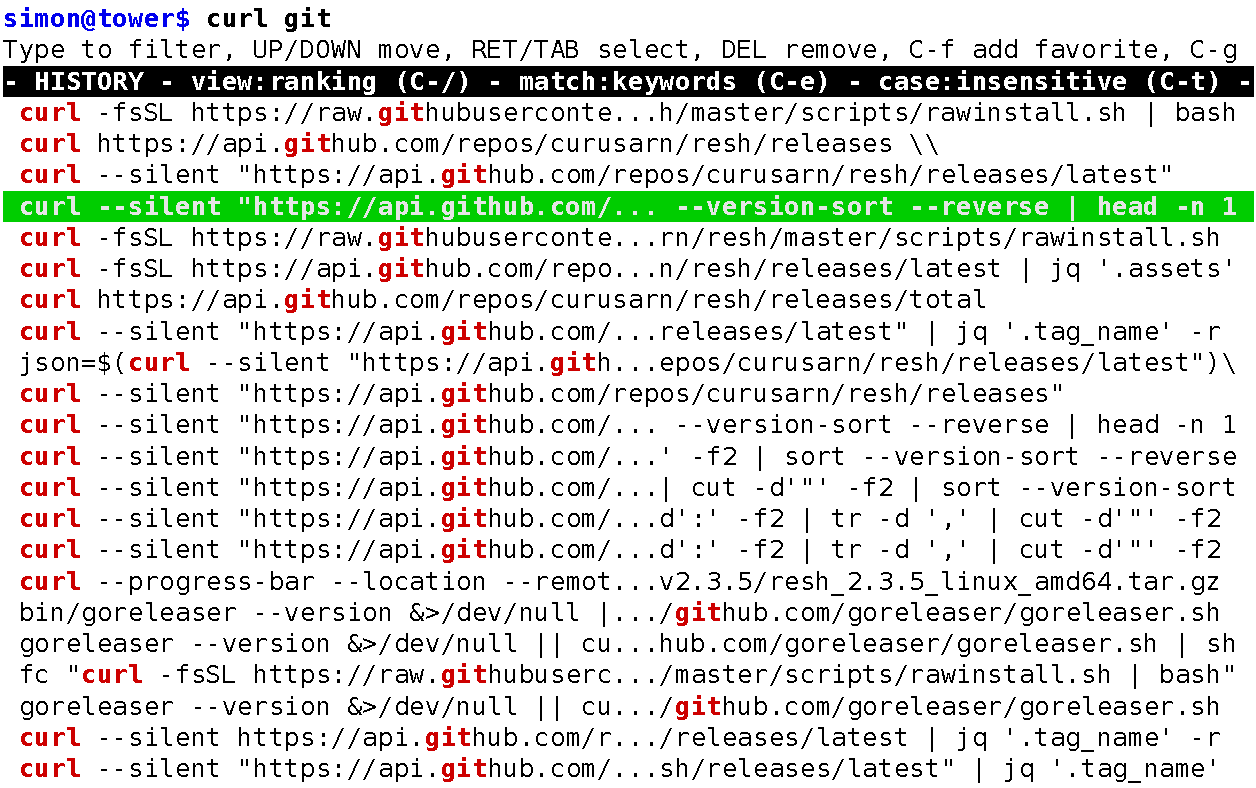
\includegraphics[width=0.995\linewidth]{figures/existing-tools/xterm-hstr-std.pdf}}
  \caption{Hstr interactive history search}
  \label{hstr-screenshot}
\end{figure}


\subsection{Fuzzy history search}

Fzf\cite{tools-fzf} is a popular\footnote{Fzf has over twenty eight thousand stars on GitHub.} general-purpose command-line fuzzy finder. The documentation of the project recommends several ways that can be used to interactively search shell history.

Searching history using Fzf addresses the issues of the history reverse search. 
Like Hstr, Fzf can display a full page of results from history. 

Fuzzy search allows Fzf to retrieve both exactly and approximately matching history entries. Exact and close matches are returned first and additional matches are returned after. 

This essentially provides a functionality of multi-query search. In addition, fuzzy search can match the desired history result even when you make typos in the query. Unlike "keywords" matching, fuzzy matching is tolerant to mistakes and typos; Naturally, this is very appealing to users. 

Fuzzy search is a commonly requested feature in various history tools. Some people who are already using Fzf cannot imagine using history tools without fuzzy search.

% \begin{figure}\tmpframe{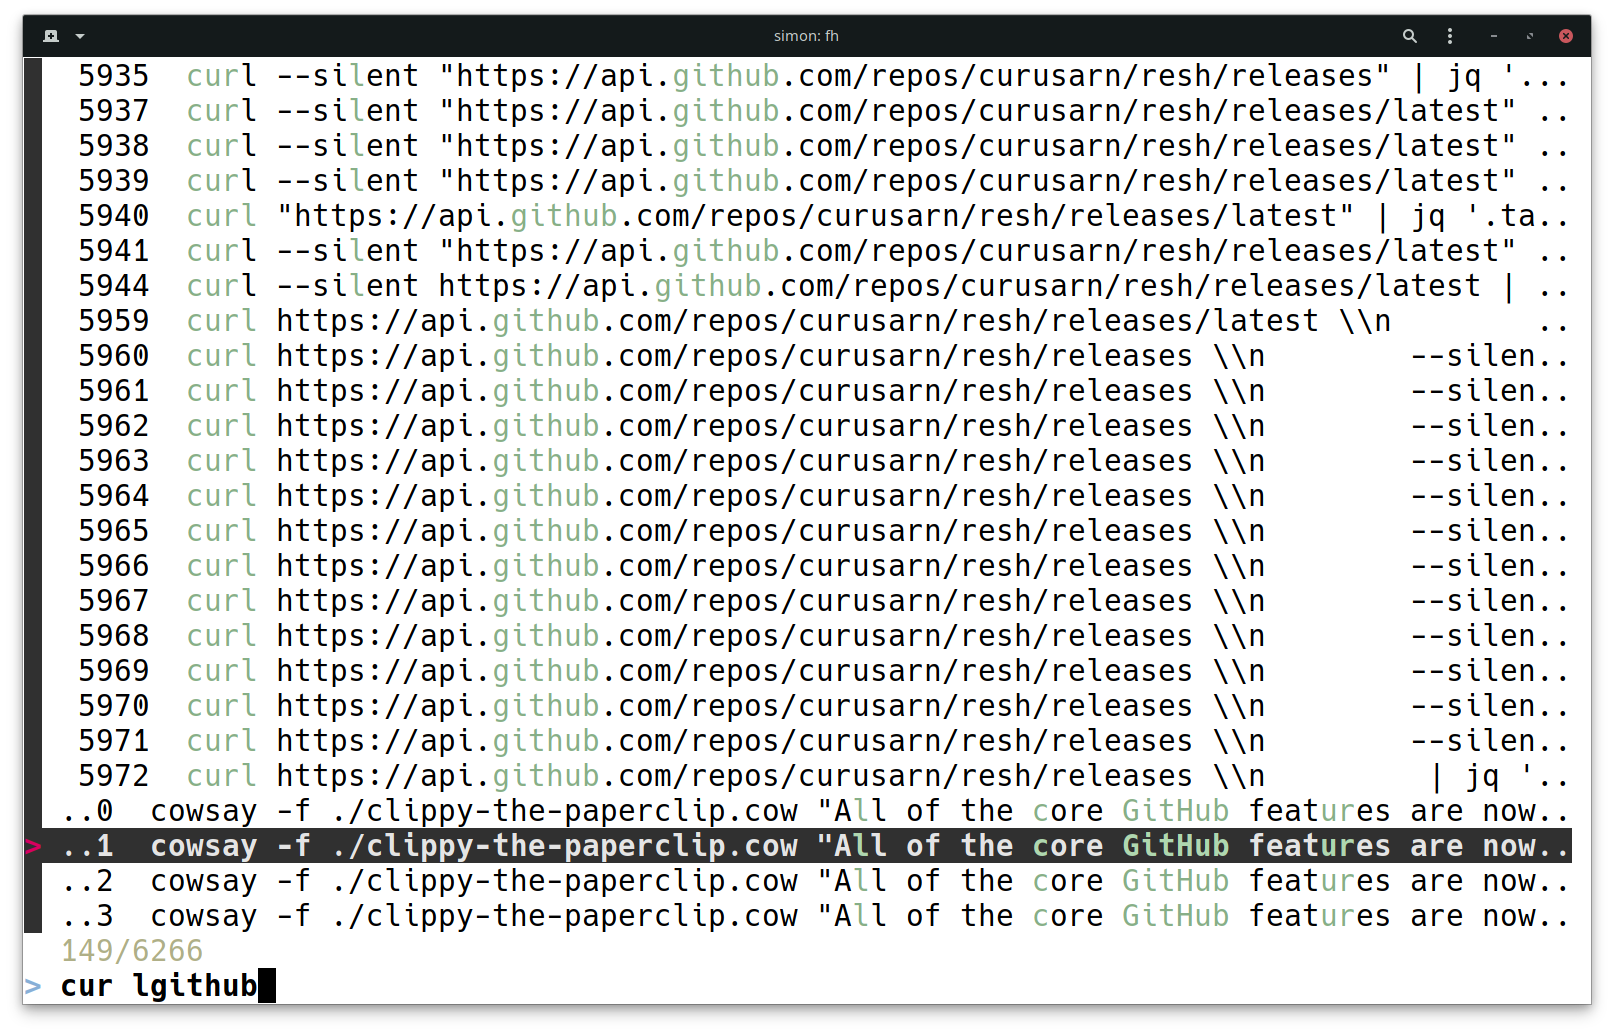
\includegraphics[width=\linewidth]{figures/existing-tools/fzf-fh-screenshot.png}}\caption{Searching history interactively using Fzf}\end{figure}

\begin{figure}
  \permanentframe{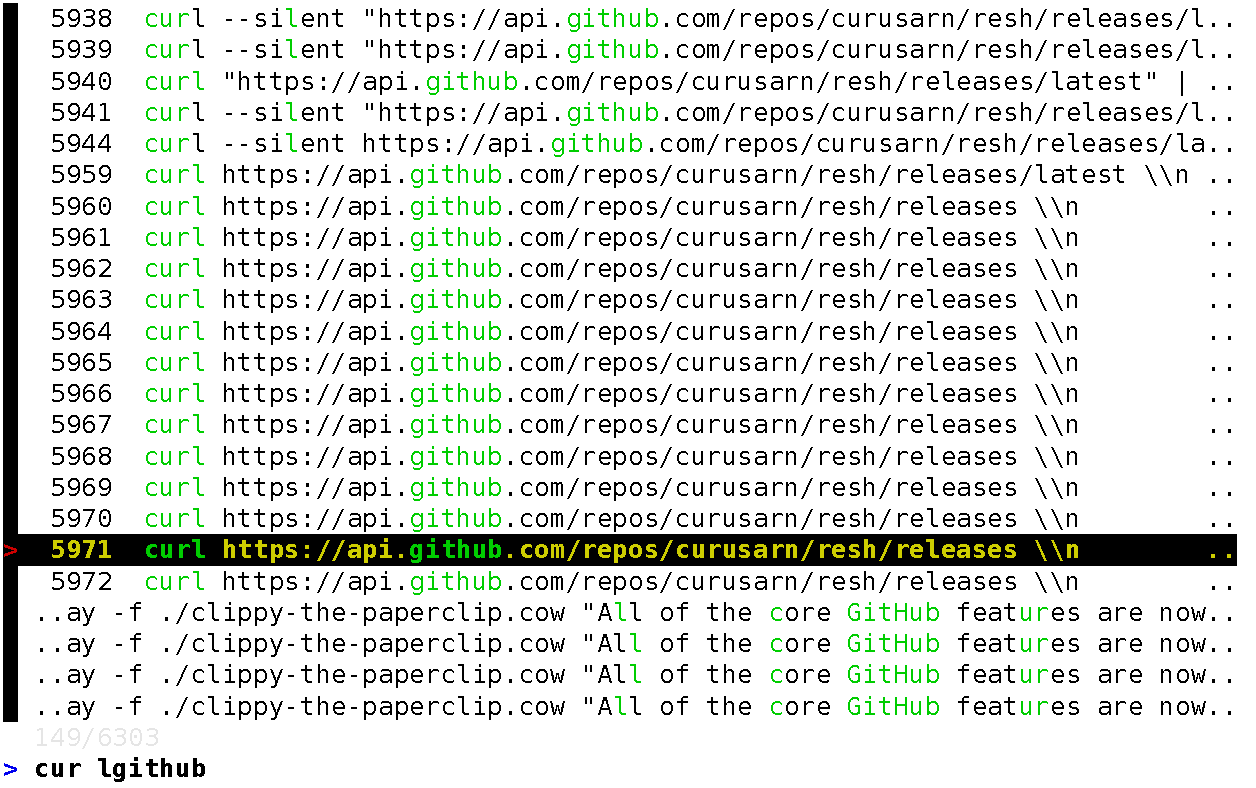
\includegraphics[width=0.995\linewidth]{figures/existing-tools/xterm-fzf-std.pdf}}
  \caption{Searching history interactively using Fzf}
\end{figure}


%\subsection{Per directory history}

%The idea behind per directory history is that your history is grouped based on directories. In practice, this means that each directory has a separate history file. 
%Since this is reasonably easy to set up, we can find many mentions, configurations, and even smaller projects that do save history to a separate file for each directory.


%Different smaller projects
%People do this even when it means not being able to reverse search the entire history.

%% https://github.com/jimhester/per-directory-history  123 gh stars
%provides switching (keybinding) between global and directory history


\subsection{Contextual shell history in the cloud}


Bashhub\cite{toolsbashhubclient} saves your shell history to the cloud and allows you to search it from all of your machines.

Apart from the command line entry, Bashhub records and saves additional context. Each history record contains following:
\begin{itemize}
    %\setlength\itemsep{0em}
    \item command line entry
    \item exit status
    \item present working directory
    \item host
    \item time of execution
    \item ID of the session
    \item ID of the record
\end{itemize}

The Bashhub history search uses pattern matching\footnote{The pattern matching is implemented using SQL "LIKE" operator.} to search the submitted command line entries. The search can be restricted to current directory and to current host.


All searching is server-side; This means that every time you search your history using Bashhub it needs to send a requests to a remote server.
These requests take time so there is no interactive "search as you type" functionality. Instead, you always have to type out the full query, execute the search command, and then wait%\footnote{Bashub server response takes about three seconds on my system.} other 
for the results. Below, you can see an example of search command that is restricted to the current directory. 

\begin{verbatim}
    bh -d "curl git"
\end{verbatim}

An obvious disadvantage of server-side search is that it does not work offline. 
When you use Bashhub, your history is saved on the remote server and the server needs to be able to search it. This means that the history is on the server, at least in memory, in an unencrypted form. Adding client side encryption would break the server-side search.

By default, the remote server is an instance maintained by the project author. The official server implementation is closed source. This means that you need to trust the author of the project with the access to your shell history. 

Recently\footnote{Open source implementation of Bashhub server was written in February 2020.} a new open source implementation\cite{toolsbashhubserver} of the Bashhub server has appeared. This addresses the privacy and security issues by making it possible to run and use your own instance of the server.

%\redtext{Bashhub is somewhat popular on GitHub\footnote{Bashhub has 744 "stars" on GitHub.}
%Bashhub is not a viable replacement for standard reverse search and manual history searching.}

%ALT sample: There is an additional open source implementation of Bashhub server available.
%ALT sample: This makes it possible to self-host instead of trusting the someone with your shell history.


% bashhub library
%\redtext{Mention https://github.com/rcaloras/bash-preexec library ??? I don't think so}

\subsection{Contextual history search powered by a neural network}

McFly\cite{toolsmcfly} is a tool that tries to predict your next command line entry using a small neural network. It predicts the next command line entry based on following contextual information:
\begin{itemize}
    \item present working directory
    \item previous command line entries
    \item how often you run the command line entry
    \item the last time you ran the command line entry
    \item if you selected the command line entry in McFly before
    \item exit status
\end{itemize}

Unlike Bashhub, this tool is designed to be bound to \verb|CTRL-R| and to replace the standard reverse search. Pressing \verb|CTRL-R| launches McFly full screen terminal app shown in figure \ref{tools-mcfly}. At first, the app displays a list of ten predicted history entries. The list of history entries is updated as you type to only show results that exactly match the typed query. The list always contains ten results or less which is a curious design decision. 


\begin{figure}[h]
  \permanentframe{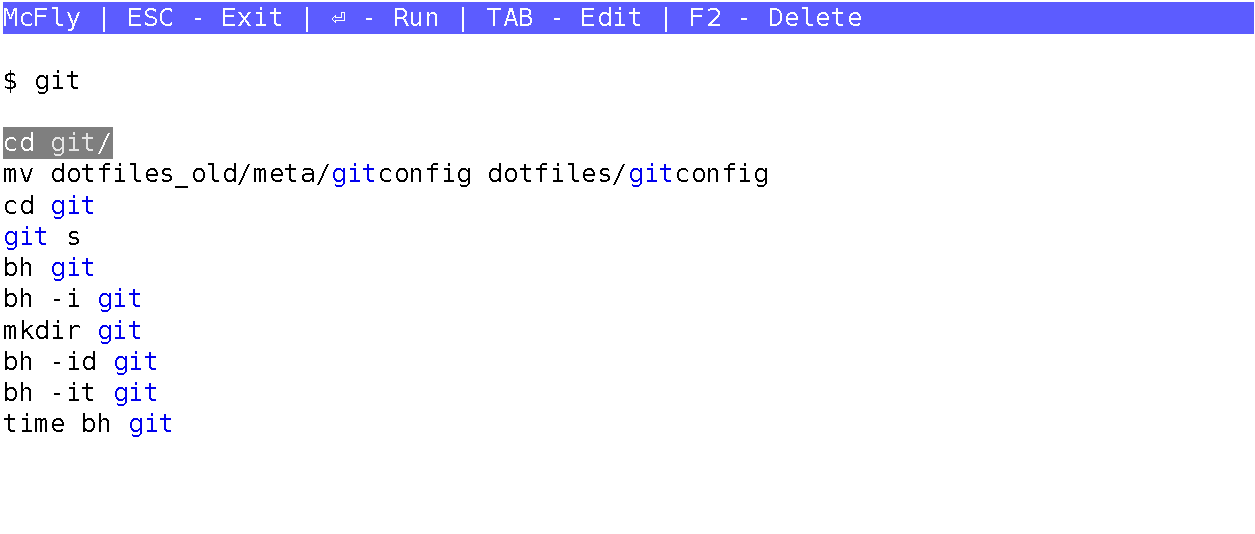
\includegraphics[width=0.995\linewidth]{figures/existing-tools/xterm-mcfly-std-short.pdf}}
  \caption{McFly interactive history search (cropped)}
  \label{tools-mcfly}
\end{figure}


When trying to use McFly we found its behavior to be unpredictable; Not knowing why specific results are being shown made the tool less useful. 

McFly also shares some problems with reverse search, it only uses a single query for searching; This can make it hard to find what you need in situations when you are unable to think of a better query\footnote{We already described such situation in section \ref{workflow-search-w-limited-knowledge}}. 

%\redtext{McFly is popular on GitHub.\footnote{McFly has about sixteen hundred "stars" on GitHub.}}

%\begin{figure} \permanentframe{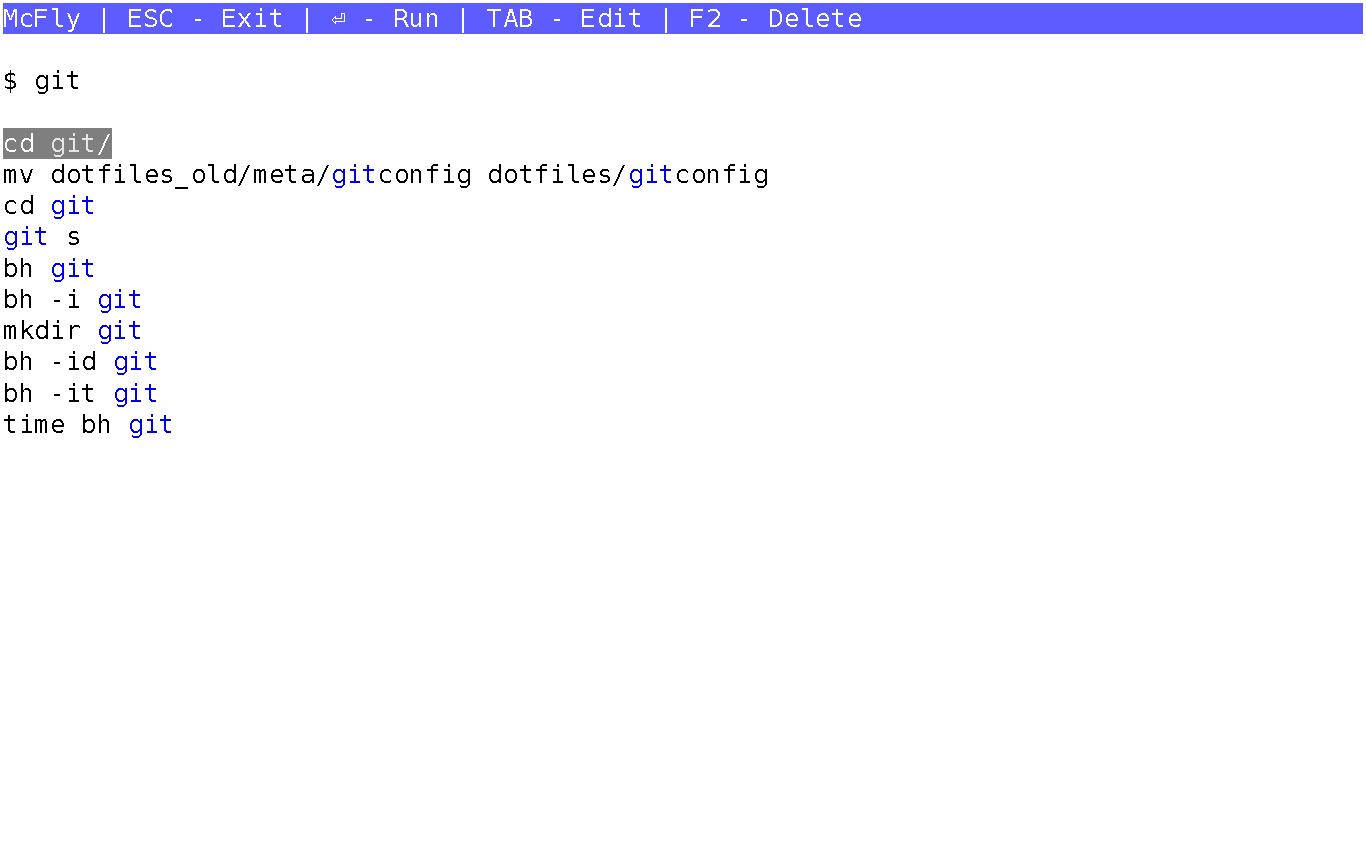
\includegraphics[width=0.995\linewidth]{figures/existing-tools/xterm-mcfly-full.pdf}}  \caption{McFly interactive history search \redtext{REMOVE IMAGE}} \end{figure}


\section{Usefulness of contextual information}

% rewrite

In previous section we talked about existing history tools. We saw that contextual history tools are not automatically more useful than tools that do not work with additional context. 

Useful history tools address real workflows and provide value to the user.
In this section, we explore available contextual information. We will discuss how different parts of the context relate to shell usage and history usage. %We do this to identify the usefulness of different parts of available contextual information. 
We cover following parts of the available contextual information:

\begin{itemize}
    \item Exit status
    \item Directory and Git related context
    \item Sequential relationships, sessions, and time
    \item Host and portability of history entries
    \item Usage of history features
\end{itemize}

\subsection{Exit status}

Zero exit status is interpreted by the shell as success; In contrast, non-zero status indicates failure.\cite{bashman} People often immediately edit and resubmit command line entries that returned an error. However, people probably rarely want to repeat older command line entries that failed. Does this mean that we can use exit status to filter out errors and only serve successful history entries to the user?

Not really, exit status does not directly map to success and failure. Programs can fail without returning an error. Some programs return non-zero exit status without actually failing\footnote{For example, GNU Grep returns one when no lines were matched and two to indicate errors.\cite{man-grep}}. 
Additionally, even history entries that are technically errors can be useful to the user. For example, the user might interrupt a program using \verb|CTRL-C| after it has fulfilled its purpose.
% We could ADD: logical errors

Generally, it is reasonable to assume that people retrieve history entries with zero exit status more often than the ones with errors. However, given the caveats described above, we should excercise this assumption conservatively. Removing history entries based on exit status would prevent the user from retrieving them. To preserve this ability we can display all history entries but prioritize the successful ones.


%In addition to exit status, there is \verb|$pipestatus| shell variable. Pipestatus gives us additional information about exit status of commands in a pipeline; Pipeline is a sequence of commands connected by shell pipes. Pipestatus is an array of exit statuses of individual commands that make up the pipeline.\cite{bashman}\cite{zshdocs} Pipelines that return zero exit status can still contain failed commands\footnote{\redtext{pipefail (both bash and zsh)}}. History entries with even one failed command in the pipeline can be treated as unsuccessful.
 
%PIPESTATUS (bash)
%An array variable (see Arrays) containing a list of exit status values from the processes in the most-recently-executed foreground pipeline (which may contain only a single command).

%pipestatus <S> <Z> (zsh)
%An array containing the exit statuses returned by all commands in the last pipeline.

\subsection{Directory and Git related context}

Directories provide explicit context; People change into different directories to complete different tasks.\cite{greenberg1993computer} It is often more comfortable to change directories compared to using longer paths as arguments. 

Many standard tools encourage the user to use specific directories for specific tasks. 
For example, Makefile, Vagrantfile, and Dockerfile are all designed to be used from within their directory\cite{man-make}\cite{docs-vagrantfile}\cite{docs-dockerfile}. 

Directories often hold projects that are associated with specific workflows and command line entries. 
These projects often use Git or other version control system; This almost forces the user to use command line entries specific to the project inside the version control repository. 

We should make it easy to access the history entries from the present working directory.
However, we do not have to stop there. Directories and Git repositories are closely related but they are not quite equivalent. Git provides some more context we can use. 
%The goal is to differentiate between history entries executed inside and outside the Git repository. 
Root of the Git repository allows us to group all history entries from the Git repository.
Git remotes\footnote{Remotes are remote repositories tracked by Git. Origin is the default remote.} can be used to identify the repository even across different machines or when it is moved to a different directory. 




\subsection{Sequential relationships, sessions, and time}

% In this section, we cover a part of context that is not well understood yet. captur

Command line entries are generally not executed individually; They are a part of longer sequences and tasks.\cite{greenberg1993computer} Each entry is related to its preceding and following command line entries. 

When analyzing shell history we collected from people, we observed significant sequential dependencies between command stubs; These dependencies represent workflows that users recognize and remember.\footnote{This specific analysis can be found in appendix in section \ref{seq-app}.}

Apart from immediate sequential dependencies, each command belongs to a terminal session. We have observed significant differences between how people use sessions; Some people often create new terminals even for a few command line entries and then close them. Others keep terminals open for a long time and reuse them for different tasks.
Additionally, people very often switch back and forth between multiple open terminals. Command line entries from simultaneous terminal sessions are usually different but all related to the same task.

These relationships between history entries and sessions are definitely interesting and possibly useful. To illustrate, imagine you type a command line entry that you already executed five times in the past. Maybe it is related to a specific task and to complete it you will need similar commands as before. Situations like this one show us the potential usefulness of session and history entry relationships.

However, it is not obvious if these relationships are general enough to be useful in the average case. It is unclear how to use this complex contextual information to provide value to the user. It is beyond the scope of this work to study the relationships between history entries and between sessions.


Nevertheless, not all of the sequential contextual information is difficult to interpret and use. Sequences of history entries are useful because there are situations when people want to repeat them\footnote{We saw such situation in section \ref{workflow-repeating-a-sequence} earlier}. We should support such workflows.
%Since sequences of history entries are directly related to a workflow we identified earlier\redtext{REF: sequential workflow} we should use the sequential property in our design. 

One more use for sequences of command line entries is recording them as a full non-deduplicated transcript. Having a full transcript of your actions gives you the ability to refer back to what you were doing earlier. A transcript of command line entries should also include the time of execution for the individual entries.
% NOT an auditing tool

%Having access to a full sequential history\footnote{Standard shell history is often deduplicated. Full sequential history is a shell history that is not deduplicated.} that represents a transcript of your actions also has its value.

\subsection{Host and portability of history entries}

Imagine that you have your shell history synchronized between multiple devices.
Each of the devices is at least a little bit different so it is a good idea to be able to tell them apart. Devices usually have hostnames we can use to identify them. 

Since each device can be different we should look at the possible differences that are relevant to the shell history. Different operating systems use different package managers to install software. For example, Debian-based distributions use Apt, Arch-based distributions use Pacman, and on MacOS people use Homebrew. Commands for one package manager will not work with others.

Many history entries are valid in both Bash and Zsh but not all history entries. Shell configuration might differ between devices which could cause some history entries to not work on all devices properly. A good example are specific shell aliases that the user added to one of their devices.

% installed software

We just described why some history entries will not work when executed from a different device. Some history entries might not work even when executed on the same device but out of the original context. Examples of this are shell variables and relative paths; Variables that were set at the time of execution can cause history entries to fail when retrieved and executed again. History entries with relative paths will only work in certain directories.

As we can see there are many reasons why history entries might not be portable. Most of the issues above can be detected using relevant contextual information. 
We could detect and handle these portability issues individually. Or alternatively we could take a simpler approach; Prioritize history entries from the current device over those from other devices. This could be effective because many of the portability issues are related to mixing shell history from different devices. 


\subsection{Usage of history features}

So far we have only described context related to the the usage of shell and to the device. Now we look at context that is related to how people use shell history. 

The first step is to know which command line entries are typed and which are retrieved from history. Next, it would be useful to know which history mechanism was used to retrieve the entry. This information is useful because people tend to repeat themselves. 
For example, when you retrieve a specific history entry using \verb|CTRL-R|, you are more likely to retrieve it using \verb|CTRL-R| again in the future. %This is supported by previous research; According to Greenberg, it should be it easy to retrieve history entries that were already retrieved earlier.\cite{greenberg1993computer}


A detailed transcript of user interactions with the history mechanisms would give us even more useful information. Consider a situation where the user presses \verb|ARROW_UP| ten times and then gives up and uses \verb|CTRL-R| to search the history instead. This is not an effective way to use history. However, it would be wrong to blame the user. If such situation happens a lot to many users we should look into if we can redesign \verb|ARROW_UP| to improve it.

The interactions between the user and the history features can help us understand how people use history. Knowing how people use standard shell history and our history solution is essential for informing design decisions. It is also crucial for evaluating the performance and usefulness of final solution. %Interactions can help us understand when the system works and when it does not.
